$subject$=Физические основы компьютерных \\ и сетевых технологий
$teacher$=Решение задач из сборника
$date$=

\begin{tcolorbox}
    \textbf{Задача 7.3.6.} Батарея из четырех одинаковых конденсаторов
    включена один раз по схеме a), а другой раз — по схеме b). 
    В каком случае емкость батареи будет больше? Если емкости 
    конденсаторов различны, то какому соотношению они должны 
    удовлетворять, чтобы при переключении со схемы a) на схему
    b) емкость батареи не менялась?
\end{tcolorbox}

\begin{center}
    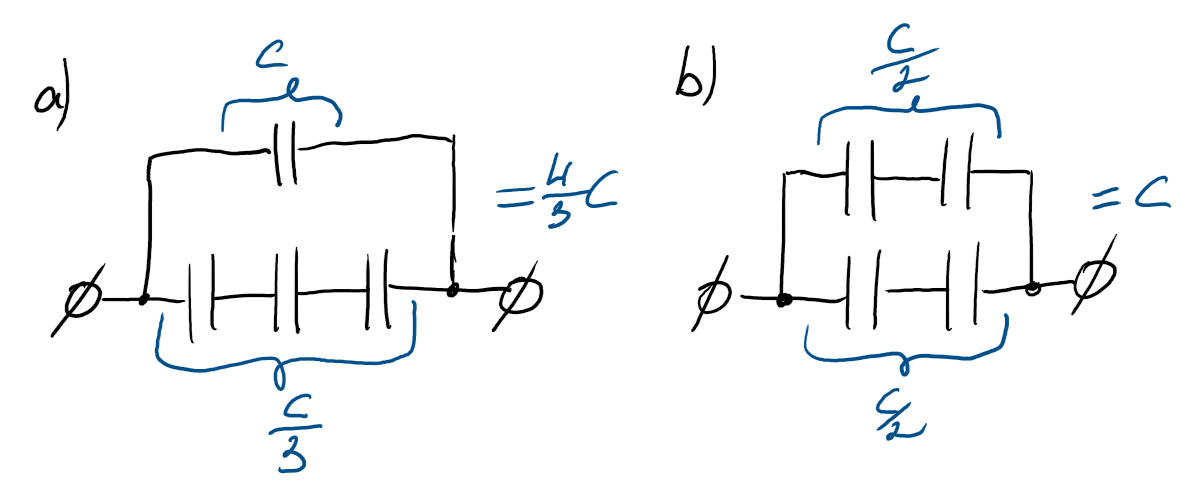
\includegraphics[width=0.9\textwidth]{physics1/images/physics1_homework_8_1}
\end{center}

Обозначим $C$ емкостью конденсатора, тогда в схеме a) нижние конденсаторы 
соединены последовательно и образуют емкость $\frac{1}{\frac{1}{C} + \frac{1}{C} + \frac{1}{C}} = \frac{C}{3}$ - 
эта группа соединена параллельна с верхним конденсатором, тогда емкость батареи - $C + \frac{C}{3} = \frac{4}{3}C$

Аналогично в схеме b) емкость батареи будет $2\left(\frac{1}{\frac{1}{C} + \frac{1}{C}}\right) = C$

Очевидно, что в схеме a) емкость больше, чем в схеме b)

\mediumvspace

Выясним, при каком соотношении емкость батареи в двух конфигурациях будет равна:

$\frac{1}{\frac{1}{C_1} + \frac{1}{C_2} + \frac{1}{C_3}} + C_4 = \frac{1}{\frac{1}{C_1} + \frac{1}{C_2}} + \frac{1}{\frac{1}{C_3} + \frac{1}{C_4}}$

$\frac{C_1 C_2 C_3}{C_2 C_3 + C_1 C_3 + C_1 C_2} + C_4 = \frac{C_1 C_2}{C_1 + C_2} + \frac{C_3 C_4}{C_3 + C_4}$

$C_1 C_2 \frac{C_3 C_1 + C_3 C_2 - C_2 C_3 - C_1 C_3 - C_1 C_2}{C_2 C_3 + C_1 C_3 + C_1 C_2} = -\frac{C^2_4}{C_3 + C_4}$

$\frac{C^2_1 C^2_2}{C_2 C_3 + C_1 C_3 + C_1 C_2} = \frac{C^2_4}{C_3 + C_4}$


\bigvspace

\underline{Ответ}: $\frac{C^2_1 C^2_2}{C_2 C_3 + C_1 C_3 + C_1 C_2} = \frac{C^2_4}{C_3 + C_4}$

\begin{tcolorbox}
    \textbf{Задача 13.9.} Четыре одинаковых конденсатора 
    соединены и присоединены к батарее с ЭДС $\varepsilon$.
    Ключ $K_2$ сначала разомкнут, а ключ $K_1$ замкнут. 
    Затем размыкают ключ $K_1$ и замыкают
    ключ $K_2$. Какова будет разность потенциалов
    на каждом конденсаторе, если ЭДС батареи
    $\varepsilon = 9$ В?
\end{tcolorbox}

\begin{minipage}{\textwidth}
    \begin{wrapfigure}{r}{0pt}
        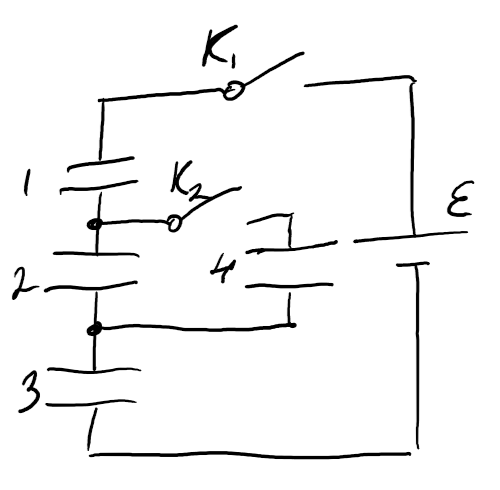
\includegraphics[width=0.4\textwidth]{physics1/images/physics1_homework_8_2}
    \end{wrapfigure}

    Ключ $K_1$ замкнут, значит через конденсаторы 1, 2 и 3 идет ток. Через конденсатор 4 ток не идет, так как ключ $K_2$ разомкнут.
    Всего емкость трех конденсаторов равна $C_{123} = \frac{C}{3}$, где $C$ - емкость одного конденсатора. Разность потенциала между ними $\varphi =$ 9 вольт,
    так как конденсаторы соединены последовательно, заряд на всех конденсаторах будет $q_1 = q_2 = q_3 = C_{123} \varphi = 3C$,
    а напряжение $U_1 = \frac{q_1}{C} = 3$ В
    
    Будем считать четвертый конденсатор незаряженным; при размыкании ключа $K_1$ ничего не происходит, при замыкании ключа $K_2$ ток пойдет
    от второго конденсатора к четвертому, причем $U_{2\text{после}} = U_{4} = \frac{U_{2\text{до}}}{2} = 1.5$ В

    Первый и третий конденсаторы не подключены в цепь, напряжение на них не изменится
\end{minipage}

\bigvspace

\underline{Ответ}: 3 В, 1.5 В, 3 В, 1.5 В

\begin{tcolorbox}
    \textbf{Задача 9.3.4.} Пространство между
    обкладками плоского конденсатора заполнено двумя
    слоями диэлектриков. Толщина слоя первого диэлектрика с
    проницаемостью $\varepsilon_1$ равна $h_1$, толщина
    слоя второго диэлектрика с проницаемостью $\varepsilon_2$ равна $h_2$. 
    Площадь каждой обкладки равна S. Найти емкость $C$ конденсатора.
\end{tcolorbox}

\begin{minipage}{\textwidth}
    \begin{wrapfigure}{r}{0pt}
        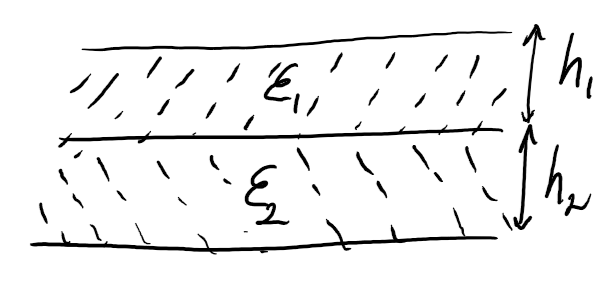
\includegraphics[width=0.4\textwidth]{physics1/images/physics1_homework_8_3}
    \end{wrapfigure}

    Считаем конденсаторы соединенными последовательно, тогда 

    $C = \frac{1}{\frac{1}{C_1} + \frac{1}{C_2}} = \frac{1}{\frac{h_1}{\varepsilon \varepsilon_1 S} + \frac{h_2}{\varepsilon \varepsilon_2 S}} = 
    \frac{1}{\frac{h_1 \varepsilon_2 + h_2 \varepsilon_1}{\varepsilon \varepsilon_1 \varepsilon_2 S}} = \frac{\varepsilon \varepsilon_1 \varepsilon_2 S}{h_1 \varepsilon_2 + h_2 \varepsilon_1}$
\end{minipage}

\bigvspace

\underline{Ответ}: $\frac{\varepsilon \varepsilon_1 \varepsilon_2 S}{h_1 \varepsilon_2 + h_2 \varepsilon_1}$

\begin{tcolorbox}
    \textbf{Задача 11.3.9.} Плоский воздушный конденсатор с пластинами
    площадью $S$ и расстоянием между ними $d$ заряжен до разности потенциалов $U$ и отключен от батареи. Какую минимальную работу
    надо совершить, чтобы увеличить расстояние между его пластинами на $\Delta x$?
\end{tcolorbox}


\begin{minipage}{\textwidth}
    \begin{wrapfigure}{r}{0pt}
        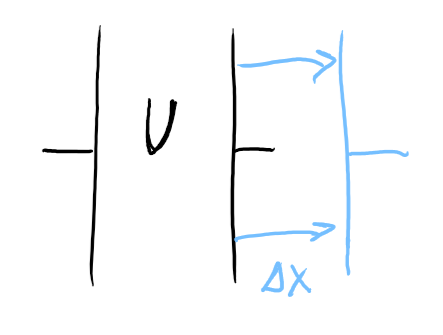
\includegraphics[width=5cm]{physics1/images/physics1_homework_8_4}
    \end{wrapfigure}

    В ходе перемещения обкладки заряд на конденсаторе не изменяется, поэтому $q = \mathrm{const} = CU = \frac{\varepsilon \varepsilon_0 S}{d} U$

    Тогда $\frac{\varepsilon \varepsilon_0 S}{d} U = \frac{\varepsilon \varepsilon_0 S}{d + \Delta x} U^{\prime}$

    Из этого $U^\prime = \frac{d + \Delta x}{d} U$

    Получаем разность напряжений $\Delta U = U^\prime - U = U\left(\frac{d + \Delta x}{d} - 1\right) = U \frac{\Delta x}{d}$

    Получаем работу $A = q \Delta U = q U \frac{\Delta x}{d} = \frac{\varepsilon \varepsilon_0 S \Delta x}{d^2} U^2$

\end{minipage}

\bigvspace

\underline{Ответ}: $\frac{\varepsilon \varepsilon_0 S \Delta x}{d^2} U^2$ Дж

\begin{tcolorbox}
    \textbf{Задача 11.3.13.} Конденсатор емкости $C_1 = 1$ мкФ ($10^{-6}$ Ф), предварительно 
    заряженный до напряжения $U = 300$ В и отсоединенный от
    источника ЭДС, подключили параллельно к незаряженному конденсатору емкости $C_2 = 2$ мкФ. 
    Найти изменение энергии этой системы к моменту установления равновесия.
\end{tcolorbox}

\begin{minipage}{\textwidth}
    \begin{wrapfigure}{r}{0pt}
        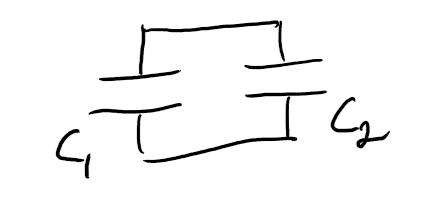
\includegraphics[width=5cm]{physics1/images/physics1_homework_8_5}
    \end{wrapfigure}

    Конденсаторы соединены параллельно, значит $U_1 = U_2$

    На первом конденсаторе до подключения ко второму сосредоточился заряд $Q = C_1 \cdot U$

    По закону сохранения заряда $q_2 + q_1 = Q \Longrightarrow C_1 U_1 + C_2 U_2 = C_1 \cdot U$

    $U_1 = U_2 = \frac{C_1}{C_1 + C_2} U$

    Энергия первого конденсатора до подключения ко второму равна $W_1 = \frac{C_1 U^2}{2} = \frac{10^{-6} \cdot 90000}{2} = 0.045$ Дж; 
    после подключения $W_2 = \frac{C_1 U_1^2 + C_2 U_2^2}{2} = \frac{C_1 + C_2}{2} \frac{C^2_1}{(C_1 + C_2)^2} U^2 = 
    \frac{C^2_1}{2(C_1 + C_2)} U^2 = \frac{10^{-12}}{2 (10^{-6} + 2 \cdot 10^{-6})} \cdot 90000 = \frac{10^{-6}}{6} \cdot 90000 = 0.015$ Дж

    $\Delta W = -0.03$ Дж

\end{minipage}

\bigvspace

\underline{Ответ}: -0.03 Дж

